\section{Mejora del algoritmo propuesto (poda de resultados)}
	\subsection{Descripción del algorítmo}

	Las podas apuntan a obviar el cálculo de soluciones que ya sabemos peores que otras ya calculadas:

	\begin{itemize}

		\item Si sabemos que en alguna rama encontramos una solución final de tamaño i y la rama actual tiene una solución parcial de $j \leq i$, podemos obviar el resto de la rama actual.

		\item Si sabemos que existe una rama con solución final 0, existe una solución óptima y no requerimos calcular nada más.

	\end{itemize}

	\begin{algorithm}[H]
		\NoCaptionOfAlgo
		
		\KwData{Lista, la lista de números a pintar}

		\KwData{UltRojo, el valor del úlitmo rojo que pintamos (si existe)}

		\KwData{UltAzul, el valor del úlitmo azul que pintamos (si existe)}

		\KwData{Indice, la posición que estamos mirando ahora (0 si recién empezamos)}

		\KwData{Actual, la cantidad de elemntos no pintados hasta ahora (0 si recién empezamos)}

		\KwData{Mejor, la mejor solución hasta ahora (el tamaño de la lista si recién empezamos)}

		\If{Actual < Mejor} {
			\uIf{Indice == $|Lista|$}{
				Llegamos al final de la lista

				Mejor es Actual
			}
			\Else{
				\If{no existe UltRojo \textbf{or} UltRojo $<$ Lista[Indice]}{
					Calcular el mejor resultado pintando de Rojo

					Llamada Recursiva: \{Lista, Lista[Indice], UltAzul, Indice+1, Res, Mejor\}

					La función modifica el valor de Mejor si corresponde
				}
				\If{Mejor $\neq$ 0}{
					\If{no existe UltAzul \textbf{or} UltAzul $>$ Lista[Indice]}{
						Calcular el mejor resultado pintando de Azul

						Llamada Recursiva: \{Lista, UltRojo, Lista[Indice], Indice+1, Res, Mejor\}

						La función modifica el valor de Mejor si corresponde
					}
					\If{Mejor $\neq$ 0}{
						Calcular el mejor resultado sin pintar

						Llamada Recursiva: \{Lista, UltRojo, UltAzul, Indice+1, Res+1, Mejor\}

						La función modifica el valor de Mejor si corresponde
					}
				}
			}
		}
	\end{algorithm}

	A diferencia del algoritmo de Backtracking básico, el orden en que se calculan los casos recursivos es importante, ya que podemos encontrar un caso óptimo y podar el resto del espacio muestral.

	\subsection{Cota de complejidad}

	El algoritmo propuesto, al igual que el algorítmo base de Backtracking, realiza hasta tres llamadas recursivas en cada paso. En mejor caso, no se realiza ninguna llamada recursiva (se realiza una poda).

	En cualquier llamada recursiva, el tamaño del problema a resolver disminuye en 1 (se avanza/pinta un solo número).

	La función de complejidad sería
	\[
	T(BTMejorado(n)) =
		\begin{cases}
			\text{1,} &\quad\text{si n == 0}\\
			\text{3 T(BTMejorado(n-1)),} &\quad\text{si no} \\
		\end{cases}
	\]

	donde n es la cantidad de números restantes, es decir, $|Lista| - Indice$.

	Es decir, en órdenes de complejidad, BTMejorado (Backtracking con podas) es igual a BT (Backtracking sin podas).

	Esto no quiere decir que las podas son irrelevantes, las mismas pueden cortar el tiempo de procesamiento de manera importante, pero los cambios en complejidad son de orden menor a $3^n$, por lo que esta sigue siendo la complejidad.

	\pagebreak
	\subsection{Gráfico de complejidad}

	El siguiente gráfico utiliza el mismo criterio que el anterior. El mismo es irregular debido a que las listas testeadas son aleatorias y por ende pueden tener mejor o peor comportamiento frente a las podas definidas.

	\begin{center}
	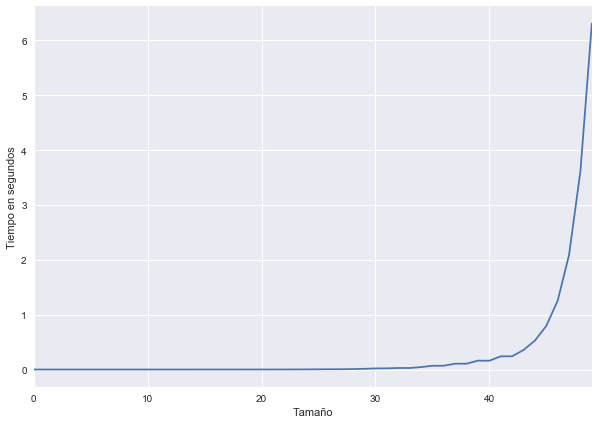
\includegraphics[width=.8\textwidth]{ej2.png}
	\end{center}

	A modo de comparación se agrega también el siguiente gráfico en el que se muestran ambos resultados en los mismos ejes, utilizando una escala logarítmica para poder comparar mejor los órdenes de complejidad. En esta escala el ruido que introducen los valores aleatorios y demás procesos en el equipo se vuelve evidente con listas pequeñas, pero a partir de 10 elementos la curva se normaliza nuevamente.

	Como evidencia el gráfico logarítmico, si bien la mejora con las podas es notoria, ambos algorítmos crecen en órdenes similares, por lo utilizar cualquiera de los dos para listas de mas de 50 elementos sigue siendo poco practicable.

	\begin{center}
	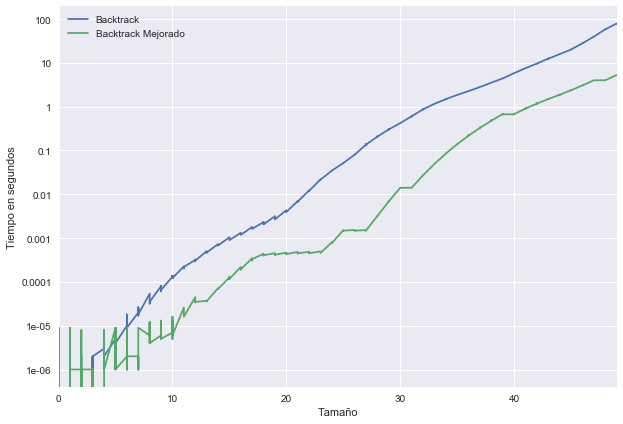
\includegraphics[width=.8\textwidth]{ej2-2.png}
	\end{center}